\appendix{Kompleksinių perturbacijų iliustracijos}
\begin{figure}[h]
    \begin{small}
        \begin{center}
            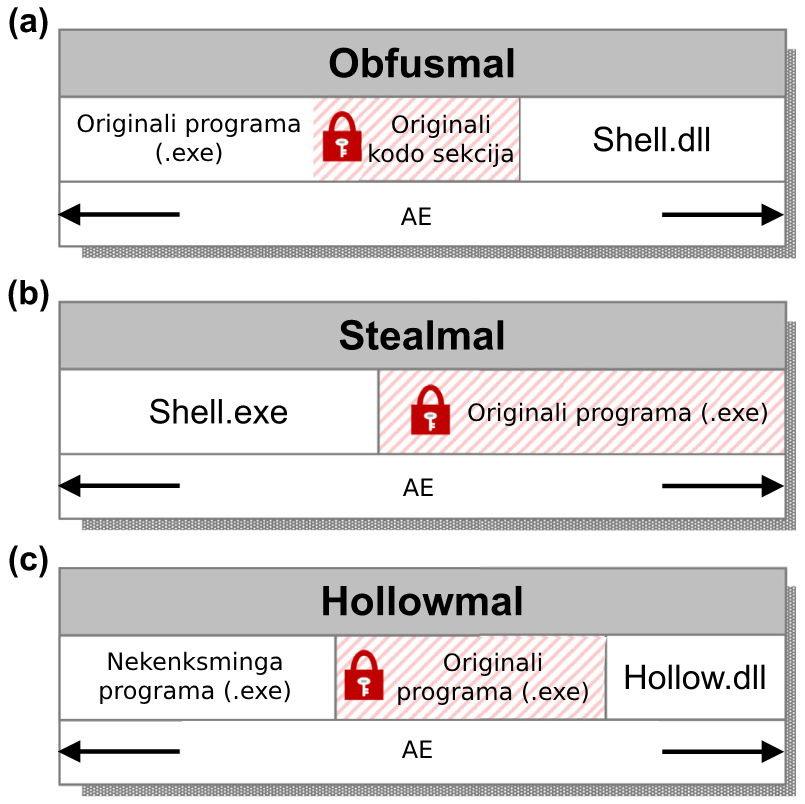
\includegraphics[width=0.95\textwidth]{img/complex-perturbations.png}
        \end{center}
        \caption{Obfusmal (a), Stealmal (b) ir Hollowmal (c) perturbacijų veikimo principų iliustracijos. Adaptuota iš \cite{zhongReinforcementLearningBased2022}}\label{fig:perturbations}
    \end{small}
\end{figure}

\appendix{Tarpiniai tyrimo rezultatai}\label{app:experiment}
\begin{figure}[h]
    \begin{small}
        \begin{center}
            \begin{subfigure}[t]{0.48\textwidth}
                \centering
                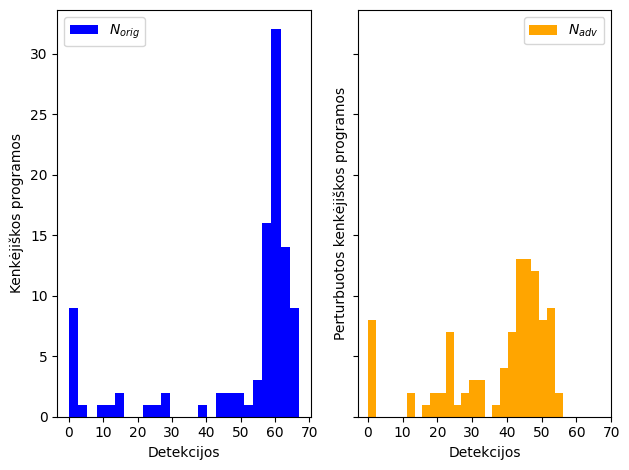
\includegraphics[width=\textwidth]{img/det_distributions_paper.png}
                \caption{\textbf{E-1}}
            \end{subfigure}
            \hfill
            \begin{subfigure}[t]{0.48\textwidth}
                \centering
                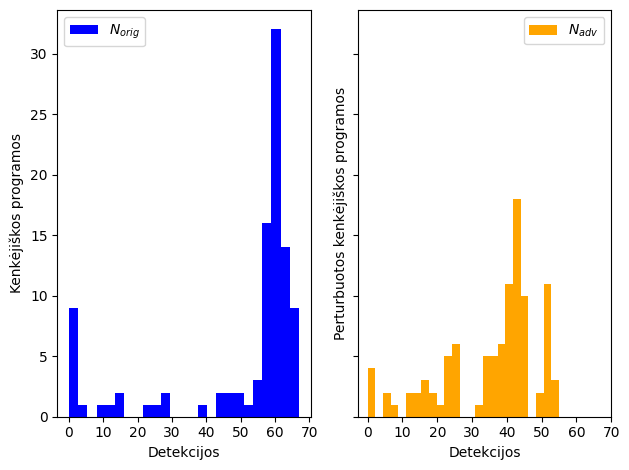
\includegraphics[width=\textwidth]{img/det_distributions.png}
                \caption{\textbf{E-2}}
            \end{subfigure}
        \end{center}
        \caption{Originalių ($N_{orig}$) ir perturbuotų ($N_{adv}$) kenkėjiškų programų detekcijų pasiskirstymas}\label{fig:experiment:det_dist}
    \end{small}
\end{figure}